% !TeX document-id = {e96318ba-ee8c-4009-b5ac-484871d58952}
% !TeX encoding = UTF-8
% !TeX program = pdflatex
% !BIB program = bibtex


%%% Um einen Artikel auf deutsch zu schreiben, genügt es die Klasse ohne
%%% Parameter zu laden.
\documentclass[english]{lni}

%%% To write an article in English, please use the option ``english'' in order
%%% to get the correct hyphenation patterns and terms.
%%% \documentclass[english]{class}
%%

\begin{document}

\title[Titlel]{Cyber-Physical-Systems and Cloud Computing}
\author[Pena Benafa]{Pena Benafa\footnote{ \email{pena.benafah@stud.hshl.de}} }
\startpage{1} % Beginn der Seitenzählung für diesen Beitrag / Start page
\booktitle{Cyber-Physical-Systems and Cloud Computing} % Name of book title
\year{Summer Term 2021}

\maketitle
\tableofcontents

\newpage

"Declaration of Originality
I hereby confirm that I have written the accompanying paper by myself, without contributions from any sources other than those cited in the text and acknowledgements.
This applies also to all graphics, drawings, maps and images included in the paper.
The paper was not examined before, nor has it been published."

\newpage

\begin{abstract}
Cyber-Physical Systems (CPS) is used to describe a combination of information processing computing systems tightly coupled with the physical world through sensors and actuators \cite{b4}.
The data from the sensors drive computation, while the actuators are used to control the physical world. CPS have been applied in smart grid, automobile systems  (Anti-lock/Anti-Skid Braking System), manufacturing, robotics, etc. Cloud computing extends the capabilities of CPS system by providing the physical and computational resources, which is often a limitation of CPS. To implement Cyber-Physical System and Cloud Computing, the CPS needs to be connected to a cloud based computing system, usually through the internet \cite{c5}. This provides the CPS with access to the enormous cloud resources and ability to share data and form system(s) with other Cyber-Physical Systems. In this seminar, an overview of cyber-physical-systems and cloud computing including some examples of simple implementations and a brief review of two research papers on the survey, applications of Cyber-Physical Systems and cloud computing will be presented. 
\end{abstract}

\newpage

\section{Motivation}
With the increased interaction between computing nodes and the physical (humans and environment), there has been growing need for more efficient power and computing methods to acquire, process and communicate data \cite{c3}. This increased interaction between computing nodes and the physical in many ways has improved the way people and environment interact with engineering systems and communicate, creating new markets, improved traffic flow, etc. However, this has led to the need for more efficient computing nodes in terms of sensors, power, computation and size. Specialized computing nodes can be balance efficiency in one domain and require some trade-offs in another domain, for example memory and computing power and size. Cyber-physical systems was birthed to address the need created by the trade-offs. With Cyber physical Systems, a computing node is specialized in performing a task \cite{a7}, for example it may contain sensors for sensing temperature, sound, light, etc and the data is sent to a remote computer that has resources for heavy computation and storage. This remote computer may also receive data from many other computing nodes with which it does its computation and sends control signals back to the nodes \cite{a7}.Thus, perception, communication, learning, behaviour or control generation can be integrated to all connected systems to achieve a great level of control in the computing nodes.

Cloud computing has gained widespread use over the years. It has become part of a business model, and it changes how businesses operate. The National Institute of Standard and Technology (NIST) defines Cloud computing as “a model for enabling ubiquitous, convenient, on-demand network access to a shared pool of configurable computing resources (e.g., networks, servers, storage, applications, and services) that can be rapidly provisioned and released with minimal management effort or service provider interaction”\cite{nist_ref}. Cloud computing, being part of the core technologies to smart society, provide a flexible platform, easy data recovery, little maintenance, quick access and a better level of security.
In recent years, Cloud facilities has been integrated into cyber-physical systems. This has birthed new fields such as Cloud Robotics and Sensor Clouds. 

\begin{figure}[ht]
    \centering
    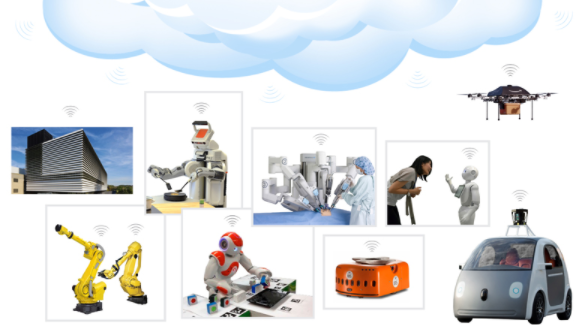
\includegraphics[width=0.65\textwidth]{Images/CloudRobotics.png}
    \caption{Cloud Robotics and Automation Illustration \cite{image1}}
    \label{fig:CloudRobtics}
\end{figure}

Cloud Robotics : Cloud robotics is an emerging study that allows CPU to offload heavy tasks to remote servers. This enables fast processing of data. With the use of cloud robotics, robots can finds an object that it's never seen or used before and get an instruction on how to use it. For example, according to professor James Kuffner, If a robot sees an object. The robot could send an image of the object to the cloud and receive back the object’s name, a 3-D model, and instructions on how to use it. Cloud robotics provides robust computation, large storage space and communications resources of modern data centres of which robots can benefit from. \cite{copyurl1}

Sensor Clouds:
Cloud sensor uses the physical sensors to accumulate its data. It collects and processes information from several sensor networks, enables information sharing on big scale, 
and collaborates with the applications on cloud among users.\cite{copyurl2}

\section{Cyber Physical Systems Conceptual Model}
The cyber physical system conceptual model shows different layers that work together in a cyber physical system. The cyber physical system  comprises different layers  or parts which work together to achieve the particular set goals. The layers include the physical layer, the network layer, the storage layer and the application layer. The figure 2 shows a model and each layer in relation to the system.

\begin{figure}[h]
    \centering
    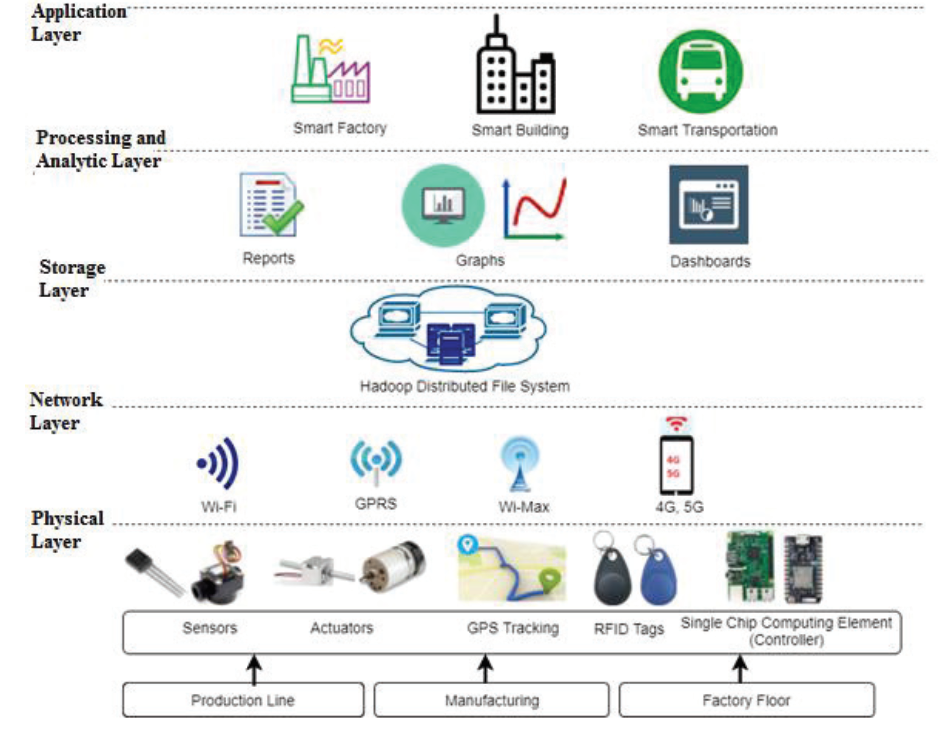
\includegraphics[width=0.65\textwidth]{Images/conceptmodel.png}
    \caption{Conceptual Model of Cyber-Physical System \cite{image2}}
    \label{fig:conceptmodel}
\end{figure}

\subsection{Physical Layer}
The physical layer is the part of the cyber-physical system that receives data from the physical environment. It consists of devices such as sensors, actuators and controllers among others.The sensor is a terminal device that first receives data from the physical environment. The data can be in various forms such as light, heat, sound, electricity etc. The sensors directly record physical data and changes the data received from the physical environment into electrical signals \cite{copyurl3}.Just like the sensor, the actuator is a terminal device. It carries out corresponding action based on the data received by the sensor. It affects physical processes \cite{copyurl3}. The controller is the part in which computation takes place. It receives and reads the data from the sensors.

\subsection{Network Layer and Storage Layer}
The Network layer is also called the transmission layer. This is the part that transmits information from the physical layer to the application layer. It offers means of communication between the physical layer and the application layer. This layer usually has both wired and wireless technologies that connects the other layers of the system and exchange of information \cite{b1}. There are different kinds of networking protocols that can be used in the network layer such as Wi-Fi, Bluetooth, infra-red and the 4G/5G network among others \cite{image2}.
The storage layer is the part where the information is stored before being transmitted to the application layer. The data can be stored in a local server or in the cloud \cite{image2}.

%\subsubsection{Wi-fi}
%\subsubsection{4G/5G} 

%\subsubsection{Distributed File System}

\subsection{Application Layer}
 In this layer, further processing and filtering of the information are carried out. The information is then used  to create smart applications. Applications of the cyber physical system are being developed in order to attach smart features to different kinds of physical systems and environment \cite{b2}. These applications will lead to the improvement in the particular areas of application. There are different areas or sectors of life where the cyber physical system can be put into practical used to solve targeted  problems. The application of the Cyber physical system to the real world  can be seen in various application scenarios. An application scenario refers to any situation where a cyber physical  and cloud computing system is actually being used. Cyber physical systems can be applied in many areas of life in order to create improvement and safety of lives and properties. For example, a cyber physical system can be applied in health care delivery to ensure that it becomes a smart health care delivery whereby the quality of service delivery can be done with ease. For instance, patient's illness can be detected without the physical presence of the patient in hospital. This is why it is called a smart health care delivery. This is why the cyber physical system should be embraced in all aspects of human lives. Apart from the health care delivery scenario, the cyber physical and cloud computing system can be used in other areas of life like in the disaster management scenario. Apart from the application scenarios, another way of analysing the application of the Cyber physical system is through application use-Cases. An application use case shows the various actors  and systems involved in the particular scenario \cite{a7}. The actors are the users engaged in the system like services providers and beneficiaries. For example, considering a scenario of smart telecommunication system, the actors include the network service providers, the end users and government regulatory agencies charge with the responsibility of monitoring and sanitization of the communication industry as the case may be. The use case for this scenario of telecommunication system also shows the different cyber physical and cloud computing  systems being used, how the actors and subsystems interact.

%\subsubsection{Application Scenario}
%\subsubsection{Application Use-Cases}

\section{Requirements and Characteristics}
Based on the sensitive nature of the cyber physical system, there are  requirements and characteristics that need to be taken into consideration. One of the characteristics is Real Time Operation. There is the need for all the components of the system to have the required capacity needed to perform the expected tasks as required in order to avoid failure which will definitely cause damage  to lives and properties \cite{copyurl3}. Another requirement worthy of note is referred to as Big Data Transport. Cyber physical system should be able to  handle the collection, transmission and distribution of large volumes of data. In addition, reliability is another important requirement for cyber physical systems. Reliability is the ability of the  system  and its various components to carry out their respective functions  accurately as expected.
Most application has medium reliability requirement e.g a smart water network while others have high reliability requirement e.g a self-driving car \cite{b2}.  A cyber physical system should have a standardized interface. It is essential to have a standard for the interface among the different users of the  Cyber physical and cloud systems. For example, the web interface is not specifically designed for smartphones or mobile devices, so it causes an overhead in the system \cite{copyurl2}. Security and privacy cannot be neglected when it comes to the cyber physical system. So much information are handled by such a system, therefore certain information should be kept private and secured. Hackers should be prevented by all means from gaining access to information that passes through or being  stored in any cyber-physical system. Social Interaction is another vital requirement for any successful cyber-physical system. The world is really a global village, so users involved in any cyber-physical system should be able to interact and share information where and when necessary. Clock Synchronization should also be taken into the scheme of things when building a cyber-physical system because timing is very important. The time a particular component uses to  complete a given task may be different from the time another component in the system will perform its own task. So there is need for proper synchronization of actions to avoid malfunctioning of the system which can lead to damage to lives and properties.

\section{Challenges of Cyber Physical System and Cloud Computing}
Cloud computing can simply be defined as means of having access to many applications and data from any network-connected device \cite{b3}.

\begin{figure}[h]
    \centering
    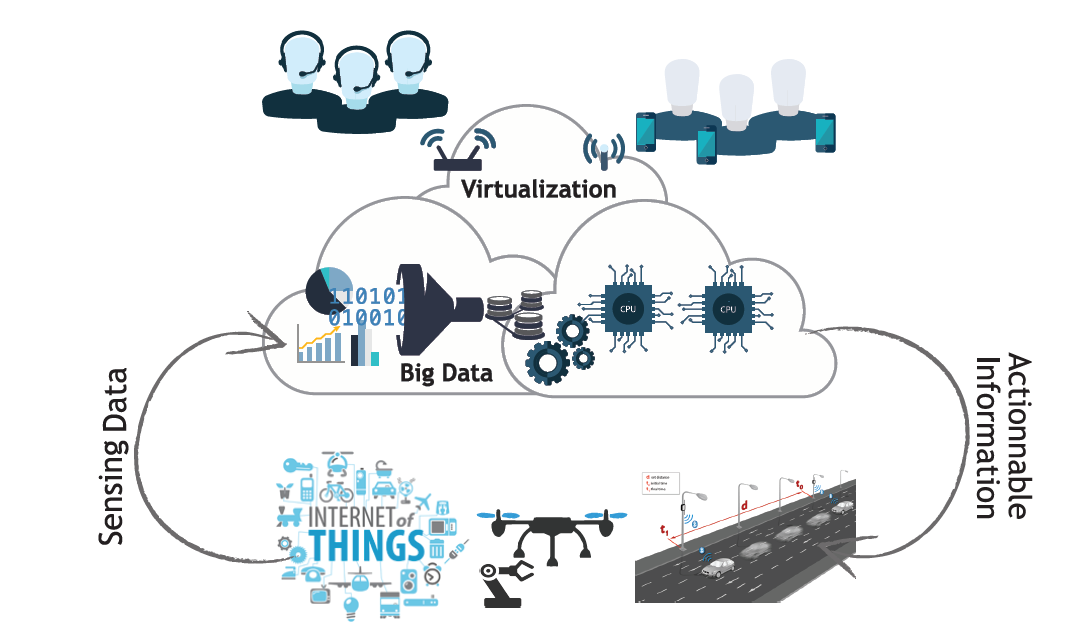
\includegraphics[width=0.65\textwidth]{Images/cpss.png}
    \caption{Cyber-Physical System Cloud \cite{b3}}
    \label{fig:cpss}
\end{figure}
Combining the cyber physical system together with cloud computing is really a good development in technology, but it poses some challenges which need to be taken into consideration in order to achieve success.
Cyber physical and cloud computation system consist of different parts and components that are connected together. It is not really easy connecting this various components together which so, care should be taken in order to carry out proper connection in the system. Such challenge is called inter-connectivity.
Apart from inter-connectivity, data integration is another challenge that should be taken care of. Data flows from one component to another, so there is need for data which is transferred from one component or system to be compatible when it gets to another component or system. A lot needs to be taken into consideration in order to achieve this particular objective otherwise, the system will not be efficient as desired \cite{b3}. Performance is really key when it comes to cyber-physical and cloud computing system. It is imperative for the various components and systems involved  to perform as expected and in order to achieve this, the proper materials and components with the required specification should be selected and used in the system without any form of compromise or neglect. Reliability is indeed paramount and worthy of mention. Each part and components of the system should be able to perform as expected. For example, any failure that occurs in the cyber physical system can lead to the damage to the system, which can cause harm to lives and damage to properties \cite{copyurl3}. Another challenge is to ensure total security and privacy of data in the system. The Cyber physical and computation cloud system handles so much information that needs to be protected as it is being transmitted from one point to another in the system.  Such information need to be protected from attacks of any form. It is very important for standards to be set in order for the cyber physical system and cloud computing to be generally accepted \cite{b3}.

%\section{Review of two Research Papers On CPS and Cloud Survey}

\section{Conclusion}
No doubt, this technology involving the cyber physical and cloud computing systems is a welcome development that must be embraced and  applied in all spheres of human lives. This paper focuses on the cyber physical system, which is a system that links the physical world to the virtual world. It has different parts that work together. The cyber physical system alone cannot be effective as expected, that is why this review also discussed the importance of cloud computing and how it is being integrated to work together with the cyber physical system in order to achieve the desired results when building smart systems to improve and protect lives and properties in the environment. Various requirements for such a system were also outlined and different  challenges facing the cyber physical and cloud computing systems were also discussed in this paper. Cyber-physical system and cloud computing technology is really a way of making life easier and better if properly done.

%%% Angabe der .bib-Datei (ohne Endung) / State .bib file (for BibTeX usage)
\bibliography{mybibfile} %\printbibliography if you use biblatex/Biber
%\bibliography{dump} %\printbibliography if you use biblatex/Biber
\end{document}




